\documentclass[twoside]{book}

% Packages required by doxygen
\usepackage{fixltx2e}
\usepackage{calc}
\usepackage{doxygen}
\usepackage[export]{adjustbox} % also loads graphicx
\usepackage{graphicx}
\usepackage[utf8]{inputenc}
\usepackage{makeidx}
\usepackage{multicol}
\usepackage{multirow}
\PassOptionsToPackage{warn}{textcomp}
\usepackage{textcomp}
\usepackage[nointegrals]{wasysym}
\usepackage[table]{xcolor}

% Font selection
\usepackage[T1]{fontenc}
\usepackage[scaled=.90]{helvet}
\usepackage{courier}
\usepackage{amssymb}
\usepackage{sectsty}
\renewcommand{\familydefault}{\sfdefault}
\allsectionsfont{%
  \fontseries{bc}\selectfont%
  \color{darkgray}%
}
\renewcommand{\DoxyLabelFont}{%
  \fontseries{bc}\selectfont%
  \color{darkgray}%
}
\newcommand{\+}{\discretionary{\mbox{\scriptsize$\hookleftarrow$}}{}{}}

% Page & text layout
\usepackage{geometry}
\geometry{%
  a4paper,%
  top=2.5cm,%
  bottom=2.5cm,%
  left=2.5cm,%
  right=2.5cm%
}
\tolerance=750
\hfuzz=15pt
\hbadness=750
\setlength{\emergencystretch}{15pt}
\setlength{\parindent}{0cm}
\setlength{\parskip}{3ex plus 2ex minus 2ex}
\makeatletter
\renewcommand{\paragraph}{%
  \@startsection{paragraph}{4}{0ex}{-1.0ex}{1.0ex}{%
    \normalfont\normalsize\bfseries\SS@parafont%
  }%
}
\renewcommand{\subparagraph}{%
  \@startsection{subparagraph}{5}{0ex}{-1.0ex}{1.0ex}{%
    \normalfont\normalsize\bfseries\SS@subparafont%
  }%
}
\makeatother

% Headers & footers
\usepackage{fancyhdr}
\pagestyle{fancyplain}
\fancyhead[LE]{\fancyplain{}{\bfseries\thepage}}
\fancyhead[CE]{\fancyplain{}{}}
\fancyhead[RE]{\fancyplain{}{\bfseries\leftmark}}
\fancyhead[LO]{\fancyplain{}{\bfseries\rightmark}}
\fancyhead[CO]{\fancyplain{}{}}
\fancyhead[RO]{\fancyplain{}{\bfseries\thepage}}
\fancyfoot[LE]{\fancyplain{}{}}
\fancyfoot[CE]{\fancyplain{}{}}
\fancyfoot[RE]{\fancyplain{}{\bfseries\scriptsize Generated by Doxygen }}
\fancyfoot[LO]{\fancyplain{}{\bfseries\scriptsize Generated by Doxygen }}
\fancyfoot[CO]{\fancyplain{}{}}
\fancyfoot[RO]{\fancyplain{}{}}
\renewcommand{\footrulewidth}{0.4pt}
\renewcommand{\chaptermark}[1]{%
  \markboth{#1}{}%
}
\renewcommand{\sectionmark}[1]{%
  \markright{\thesection\ #1}%
}

% Indices & bibliography
\usepackage{natbib}
\usepackage[titles]{tocloft}
\setcounter{tocdepth}{3}
\setcounter{secnumdepth}{5}
\makeindex

% Hyperlinks (required, but should be loaded last)
\usepackage{ifpdf}
\ifpdf
  \usepackage[pdftex,pagebackref=true]{hyperref}
\else
  \usepackage[ps2pdf,pagebackref=true]{hyperref}
\fi
\hypersetup{%
  colorlinks=true,%
  linkcolor=blue,%
  citecolor=blue,%
  unicode%
}

% Custom commands
\newcommand{\clearemptydoublepage}{%
  \newpage{\pagestyle{empty}\cleardoublepage}%
}

\usepackage{caption}
\captionsetup{labelsep=space,justification=centering,font={bf},singlelinecheck=off,skip=4pt,position=top}

%===== C O N T E N T S =====

\begin{document}

% Titlepage & ToC
\hypersetup{pageanchor=false,
             bookmarksnumbered=true,
             pdfencoding=unicode
            }
\pagenumbering{alph}
\begin{titlepage}
\vspace*{7cm}
\begin{center}%
{\Large My Project \\[1ex]\large 0.\+1 }\\
\vspace*{1cm}
{\large Generated by Doxygen 1.8.12}\\
\end{center}
\end{titlepage}
\clearemptydoublepage
\pagenumbering{roman}
\tableofcontents
\clearemptydoublepage
\pagenumbering{arabic}
\hypersetup{pageanchor=true}

%--- Begin generated contents ---
\chapter{Hierarchical Index}
\section{Class Hierarchy}
This inheritance list is sorted roughly, but not completely, alphabetically\+:\begin{DoxyCompactList}
\item \contentsline{section}{P\+Z\+M.\+puzzle\+\_\+solver.\+Puzzle\+Solve}{\pageref{class_p_z_m_1_1puzzle__solver_1_1_puzzle_solve}}{}
\item Test\+Case\begin{DoxyCompactList}
\item \contentsline{section}{P\+Z\+M.\+puzzle\+\_\+solver.\+App\+Test}{\pageref{class_p_z_m_1_1puzzle__solver_1_1_app_test}}{}
\end{DoxyCompactList}
\end{DoxyCompactList}

\chapter{Class Index}
\section{Class List}
Here are the classes, structs, unions and interfaces with brief descriptions\+:\begin{DoxyCompactList}
\item\contentsline{section}{\hyperlink{class_p_z_m_1_1puzzle__solver_1_1_app_test}{P\+Z\+M.\+puzzle\+\_\+solver.\+App\+Test} }{\pageref{class_p_z_m_1_1puzzle__solver_1_1_app_test}}{}
\item\contentsline{section}{\hyperlink{class_p_z_m_1_1puzzle__solver_1_1_puzzle_solve}{P\+Z\+M.\+puzzle\+\_\+solver.\+Puzzle\+Solve} }{\pageref{class_p_z_m_1_1puzzle__solver_1_1_puzzle_solve}}{}
\end{DoxyCompactList}

\chapter{Class Documentation}
\hypertarget{class_p_z_m_1_1puzzle__solver_1_1_app_test}{}\section{P\+Z\+M.\+puzzle\+\_\+solver.\+App\+Test Class Reference}
\label{class_p_z_m_1_1puzzle__solver_1_1_app_test}\index{P\+Z\+M.\+puzzle\+\_\+solver.\+App\+Test@{P\+Z\+M.\+puzzle\+\_\+solver.\+App\+Test}}
Inheritance diagram for P\+Z\+M.\+puzzle\+\_\+solver.\+App\+Test\+:\begin{figure}[H]
\begin{center}
\leavevmode
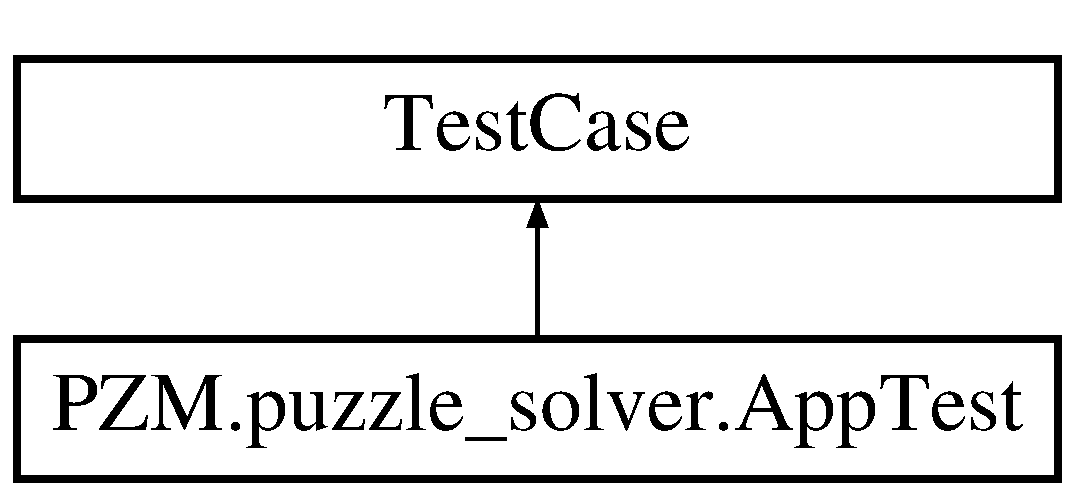
\includegraphics[height=2.000000cm]{class_p_z_m_1_1puzzle__solver_1_1_app_test}
\end{center}
\end{figure}
\subsection*{Public Member Functions}
\begin{DoxyCompactItemize}
\item 
\hyperlink{class_p_z_m_1_1puzzle__solver_1_1_app_test_a7d590d954478869ebd271bdc87d28e3d}{App\+Test} (String test\+Name)
\item 
void \hyperlink{class_p_z_m_1_1puzzle__solver_1_1_app_test_adbdc8d9da9022bad47e1a9fc26c61361}{test\+App} ()
\end{DoxyCompactItemize}
\subsection*{Static Public Member Functions}
\begin{DoxyCompactItemize}
\item 
static Test \hyperlink{class_p_z_m_1_1puzzle__solver_1_1_app_test_afff2d4eeeefe140d3b87ef7bf9022cad}{suite} ()
\end{DoxyCompactItemize}


\subsection{Detailed Description}
Unit test for simple App. 

\subsection{Constructor \& Destructor Documentation}
\hypertarget{class_p_z_m_1_1puzzle__solver_1_1_app_test_a7d590d954478869ebd271bdc87d28e3d}{}\label{class_p_z_m_1_1puzzle__solver_1_1_app_test_a7d590d954478869ebd271bdc87d28e3d} 
\index{P\+Z\+M\+::puzzle\+\_\+solver\+::\+App\+Test@{P\+Z\+M\+::puzzle\+\_\+solver\+::\+App\+Test}!App\+Test@{App\+Test}}
\index{App\+Test@{App\+Test}!P\+Z\+M\+::puzzle\+\_\+solver\+::\+App\+Test@{P\+Z\+M\+::puzzle\+\_\+solver\+::\+App\+Test}}
\subsubsection{\texorpdfstring{App\+Test()}{AppTest()}}
{\footnotesize\ttfamily P\+Z\+M.\+puzzle\+\_\+solver.\+App\+Test.\+App\+Test (\begin{DoxyParamCaption}\item[{String}]{test\+Name }\end{DoxyParamCaption})}

Create the test case


\begin{DoxyParams}{Parameters}
{\em test\+Name} & name of the test case \\
\hline
\end{DoxyParams}


\subsection{Member Function Documentation}
\hypertarget{class_p_z_m_1_1puzzle__solver_1_1_app_test_afff2d4eeeefe140d3b87ef7bf9022cad}{}\label{class_p_z_m_1_1puzzle__solver_1_1_app_test_afff2d4eeeefe140d3b87ef7bf9022cad} 
\index{P\+Z\+M\+::puzzle\+\_\+solver\+::\+App\+Test@{P\+Z\+M\+::puzzle\+\_\+solver\+::\+App\+Test}!suite@{suite}}
\index{suite@{suite}!P\+Z\+M\+::puzzle\+\_\+solver\+::\+App\+Test@{P\+Z\+M\+::puzzle\+\_\+solver\+::\+App\+Test}}
\subsubsection{\texorpdfstring{suite()}{suite()}}
{\footnotesize\ttfamily static Test P\+Z\+M.\+puzzle\+\_\+solver.\+App\+Test.\+suite (\begin{DoxyParamCaption}{ }\end{DoxyParamCaption})\hspace{0.3cm}{\ttfamily [static]}}

\begin{DoxyReturn}{Returns}
the suite of tests being tested 
\end{DoxyReturn}
\hypertarget{class_p_z_m_1_1puzzle__solver_1_1_app_test_adbdc8d9da9022bad47e1a9fc26c61361}{}\label{class_p_z_m_1_1puzzle__solver_1_1_app_test_adbdc8d9da9022bad47e1a9fc26c61361} 
\index{P\+Z\+M\+::puzzle\+\_\+solver\+::\+App\+Test@{P\+Z\+M\+::puzzle\+\_\+solver\+::\+App\+Test}!test\+App@{test\+App}}
\index{test\+App@{test\+App}!P\+Z\+M\+::puzzle\+\_\+solver\+::\+App\+Test@{P\+Z\+M\+::puzzle\+\_\+solver\+::\+App\+Test}}
\subsubsection{\texorpdfstring{test\+App()}{testApp()}}
{\footnotesize\ttfamily void P\+Z\+M.\+puzzle\+\_\+solver.\+App\+Test.\+test\+App (\begin{DoxyParamCaption}{ }\end{DoxyParamCaption})}

Rigourous Test \+:-\/) 

The documentation for this class was generated from the following file\+:\begin{DoxyCompactItemize}
\item 
src/test/java/\+P\+Z\+M/puzzle\+\_\+solver/App\+Test.\+java\end{DoxyCompactItemize}

\hypertarget{class_p_z_m_1_1puzzle__solver_1_1_puzzle_solve}{}\section{P\+Z\+M.\+puzzle\+\_\+solver.\+Puzzle\+Solve Class Reference}
\label{class_p_z_m_1_1puzzle__solver_1_1_puzzle_solve}\index{P\+Z\+M.\+puzzle\+\_\+solver.\+Puzzle\+Solve@{P\+Z\+M.\+puzzle\+\_\+solver.\+Puzzle\+Solve}}
\subsection*{Static Public Member Functions}
\begin{DoxyCompactItemize}
\item 
static void \hyperlink{class_p_z_m_1_1puzzle__solver_1_1_puzzle_solve_a23f2fa383e45e7dcbd484108f38bcea9}{main} (String\mbox{[}$\,$\mbox{]} args)
\item 
static void \hyperlink{class_p_z_m_1_1puzzle__solver_1_1_puzzle_solve_a0a5427627d50f43c830e3c6e8f858859}{puzzle\+\_\+solve} (int k, Array\+List$<$ String $>$ S, Array\+List$<$ String $>$ U)
\end{DoxyCompactItemize}


\subsection{Detailed Description}
Clase de algoritmo de resolución de problemas 

\subsection{Member Function Documentation}
\hypertarget{class_p_z_m_1_1puzzle__solver_1_1_puzzle_solve_a23f2fa383e45e7dcbd484108f38bcea9}{}\label{class_p_z_m_1_1puzzle__solver_1_1_puzzle_solve_a23f2fa383e45e7dcbd484108f38bcea9} 
\index{P\+Z\+M\+::puzzle\+\_\+solver\+::\+Puzzle\+Solve@{P\+Z\+M\+::puzzle\+\_\+solver\+::\+Puzzle\+Solve}!main@{main}}
\index{main@{main}!P\+Z\+M\+::puzzle\+\_\+solver\+::\+Puzzle\+Solve@{P\+Z\+M\+::puzzle\+\_\+solver\+::\+Puzzle\+Solve}}
\subsubsection{\texorpdfstring{main()}{main()}}
{\footnotesize\ttfamily static void P\+Z\+M.\+puzzle\+\_\+solver.\+Puzzle\+Solve.\+main (\begin{DoxyParamCaption}\item[{String \mbox{[}$\,$\mbox{]}}]{args }\end{DoxyParamCaption})\hspace{0.3cm}{\ttfamily [static]}}

Ejecuta un ejemplo del algoritmo de resolución de problemas 
\begin{DoxyParams}{Parameters}
{\em args} & -\/ Argumentos de main que se pasan por consola (no son necesarios en este ejemplo) \\
\hline
\end{DoxyParams}
\hypertarget{class_p_z_m_1_1puzzle__solver_1_1_puzzle_solve_a0a5427627d50f43c830e3c6e8f858859}{}\label{class_p_z_m_1_1puzzle__solver_1_1_puzzle_solve_a0a5427627d50f43c830e3c6e8f858859} 
\index{P\+Z\+M\+::puzzle\+\_\+solver\+::\+Puzzle\+Solve@{P\+Z\+M\+::puzzle\+\_\+solver\+::\+Puzzle\+Solve}!puzzle\+\_\+solve@{puzzle\+\_\+solve}}
\index{puzzle\+\_\+solve@{puzzle\+\_\+solve}!P\+Z\+M\+::puzzle\+\_\+solver\+::\+Puzzle\+Solve@{P\+Z\+M\+::puzzle\+\_\+solver\+::\+Puzzle\+Solve}}
\subsubsection{\texorpdfstring{puzzle\+\_\+solve()}{puzzle\_solve()}}
{\footnotesize\ttfamily static void P\+Z\+M.\+puzzle\+\_\+solver.\+Puzzle\+Solve.\+puzzle\+\_\+solve (\begin{DoxyParamCaption}\item[{int}]{k,  }\item[{Array\+List$<$ String $>$}]{S,  }\item[{Array\+List$<$ String $>$}]{U }\end{DoxyParamCaption})\hspace{0.3cm}{\ttfamily [static]}}

Algoritmo de resolución de problemas. Retorna subconjuntos S con k elementos a partir de un conjunto base U. 
\begin{DoxyParams}{Parameters}
{\em k} & -\/ Número de soluciones. \\
\hline
{\em S} & -\/ Array de subconjunto. \\
\hline
{\em U} & -\/ Array de conjunto principal. \\
\hline
\end{DoxyParams}


The documentation for this class was generated from the following file\+:\begin{DoxyCompactItemize}
\item 
src/main/java/\+P\+Z\+M/puzzle\+\_\+solver/Puzzle\+Solve.\+java\end{DoxyCompactItemize}

%--- End generated contents ---

% Index
\backmatter
\newpage
\phantomsection
\clearemptydoublepage
\addcontentsline{toc}{chapter}{Index}
\printindex

\end{document}
